% مدار LC کلاسیک و زوج کانونی (Φ, Q)
% سبک مشترک نمودارهای سند پایه‌ها (فقط داخل محیط latin فراخوانی شود)
\tikzset{
	qafbox/.style={
		draw=black!55,
		rounded corners=2pt,
		align=center,
		inner sep=3pt,
		thick,
		fill=white,
		font=\footnotesize\linespread{1}\selectfont,
		minimum height=0.95cm
	},
	qafwide/.style={
		qafbox,
		text width=2.55cm
	},
	qafnarr/.style={
		qafbox,
		text width=2.05cm
	},
	qaftitle/.style={
		font=\small\bfseries\linespread{1}\selectfont,
		align=center
	},
	qafarr/.style={
		-{Latex[length=2.2mm]},
		thick,
		draw=black!65
	},
	qafpanel/.style={
		draw,
		thick,
		rounded corners=4pt,
		inner xsep=8pt,
		inner ysep=8pt
	}
}

\begin{tikzpicture}[
	x=1cm,
	y=1cm,
	note/.style={font=\scriptsize, text=black!60, align=center}
	]
	% inductor box
	\draw[thick] (0,0.8) -- (0,1.4);
	\draw[thick] (0,1.4) -- (0.15,1.55) -- (0.35,1.25) -- (0.55,1.55) -- (0.75,1.25)
		-- (0.95,1.55) -- (1.15,1.25) -- (1.35,1.55) -- (1.5,1.4) -- (1.5,0.8);
	\node[note] at (0.75,2.05) {$L$};
	% capacitor
	\draw[thick] (0,0.8) -- (0,0.2) -- (0.55,0.2);
	\draw[thick] (0.55,0.05) -- (0.55,0.35);
	\draw[thick] (0.75,0.05) -- (0.75,0.35);
	\draw[thick] (0.75,0.2) -- (1.5,0.2) -- (1.5,0.8);
	\node[note] at (0.65,-0.25) {$C$};

	\node[note, text width=4.2cm, align=left] at (4.6,1.0) {%
		Canonical pair:\\[2pt]
		flux $\Phi$, charge $Q$\\[2pt]
		$H=\dfrac{Q^2}{2C}+\dfrac{\Phi^2}{2L}$\\[2pt]
		quantize: $[\hat\Phi,\hat Q]=i\hbar$};
\end{tikzpicture}
